%%%%%%%%%%%%%%%%%%%%%%%%%%%%%%%%%%%%%%%%%
% Journal Article
% LaTeX Template
% Version 1.3 (9/9/13)
%
% This template has been downloaded from:
% http://www.LaTeXTemplates.com
%
% Original author:
% Frits Wenneker (http://www.howtotex.com)
%
% License:
% CC BY-NC-SA 3.0 (http://creativecommons.org/licenses/by-nc-sa/3.0/)
%
%%%%%%%%%%%%%%%%%%%%%%%%%%%%%%%%%%%%%%%%%

%----------------------------------------------------------------------------------------
%	PACKAGES AND OTHER DOCUMENT CONFIGURATIONS
%----------------------------------------------------------------------------------------

\documentclass[twoside]{article}

\usepackage{etex}
\usepackage{tikz} %graphics
\usepackage{tikz-qtree} % tree macros
\usepackage{tikz-dependency} % tree macros
\usepackage[sc]{mathpazo} % Use the Palatino font
\usepackage[T1]{fontenc} % Use 8-bit encoding that has 256 glyphs
\linespread{1.05} % Line spacing - Palatino needs more space between lines
\usepackage{microtype} % Slightly tweak font spacing for aesthetics

\usepackage[hmarginratio=1:1,top=32mm,columnsep=20pt]{geometry} % Document margins
\usepackage{multicol} % Used for the two-column layout of the document
\usepackage[hang, small,labelfont=bf,up,textfont=it,up]{caption} % Custom captions under/above floats in tables or figures
\usepackage{booktabs} % Horizontal rules in tables
\usepackage{float} % Required for tables and figures in the multi-column environment - they need to be placed in specific locations with the [H] (e.g. \begin{table}[H])
\usepackage{hyperref} % For hyperlinks in the PDF

\usepackage{lettrine} % The lettrine is the first enlarged letter at the beginning of the text
\usepackage{paralist} % Used for the compactitem environment which makes bullet points with less space between them

\usepackage{abstract} % Allows abstract customization
\renewcommand{\abstractnamefont}{\normalfont\bfseries} % Set the "Abstract" text to bold
\renewcommand{\abstracttextfont}{\normalfont\small\itshape} % Set the abstract itself to small italic text

\usepackage{titlesec} % Allows customization of titles
\renewcommand\thesection{\Roman{section}} % Roman numerals for the sections
\renewcommand\thesubsection{\Roman{subsection}} % Roman numerals for subsections
\titleformat{\section}[block]{\large\scshape\centering}{\thesection.}{1em}{} % Change the look of the section titles
\titleformat{\subsection}[block]{\large}{\thesubsection.}{1em}{} % Change the look of the section titles

\usepackage{fancyhdr} % Headers and footers
\pagestyle{fancy} % All pages have headers and footers
\fancyhead{} % Blank out the default header
\fancyfoot{} % Blank out the default footer
\fancyhead[C]{Dependency-Based QA $\bullet$ 2015 $\bullet$ CMPSCI 585} % Custom header text
\fancyfoot[RO,LE]{\thepage} % Custom footer text

\usepackage{caption}
\usepackage{amsmath}
\usepackage{stmaryrd}

%----------------------------------------------------------------------------------------
%	TITLE SECTION
%----------------------------------------------------------------------------------------

\title{\vspace{-5mm}\fontsize{18pt}{10pt}\selectfont\textbf{Dependency-Based Structures\\For Question Answering}} % Article title

\author{
\large
\textsc{Alan J. Zaffetti}\\[2mm]%\thanks{A thank you or further information}\\[2mm] % Your name
\normalsize University of Massachusetts Amherst \\ % Your institution
\normalsize \href{mailto:azaffett@umass.edu}{azaffett@umass.edu} % Your email address
%\vspace{-5mm}
}
\date{}

%----------------------------------------------------------------------------------------

\begin{document}

\maketitle % Insert title

\thispagestyle{fancy} % All pages have headers and footers

%----------------------------------------------------------------------------------------
%	ABSTRACT
%----------------------------------------------------------------------------------------

\begin{abstract}

\noindent Question answering (QA) is a notoriously difficult task, requiring massive human effort, and usually resulting in complex systems.  In this project I explore a unified, logical formalism for representing relational knowledge from natural language.  Finally, with a modest amount of human effort, I show how probabilistic QA may be done on this structure for baseline QA.  I introduce parsed dependency graphs to represent NL sentences and demonstrate how to convert these structures into logical forms using a deterministic method.  I develop baseline probabilistic techniques for answering forms of wh-questions, and finally, apply my method to an academic Wikipedia dataset (Carnegie Mellon, University of Pittsburgh).

\end{abstract}

%----------------------------------------------------------------------------------------
%	ARTICLE CONTENTS
%----------------------------------------------------------------------------------------

\section{Introduction}

\lettrine[nindent=0em,lines=3]{T}he problem of question answering is a hard one because it is composed of multiple steps all of which are imperfect, and introduce error.  It is saved only by the fact that it is modular; tasks can be broken up into smaller and less complicated subtasks.  In a question answering system, this includes the methods used to break text up into sentences or sometimes individual tokens (\textit{tokenizer}); a technique for parsing sentences into a structured form (\textit{parser}); a strategy for representing structured facts derived from these parses (\textit{knowledge representation}); and finally a way to query the representation (\textit{IR}). Of course, there are more subprocesses within these.

The modularity of a system is nice for two reasons.  (1) it reduces the complexity of the system as a whole; and (2) it makes each step accountable for its performance on the system.  You may not trust the modules individually, but are more apt to trust the system as a whole because you can always find a \textit{better} tokenizer, or a \textit{faster} parser.  The modules on my system have their limitations.  For instance, my parser module does not handle unicode, and my tokenizer is brittle, but they can always be subbed out for other, better systems.

My system hopes to accomplish baseline fact-based \textit{wh}-QA (i.e. mostly \textit{what}, but perhaps \textit{when}, \textit{where}, etc.), while providing a framework for effecient QA methods at scale. However, this paper does not describe an end-to-end system, nor is the final project meant to accomplish this goal.  Instead, I will focus on demonstrating how my system ingests parsed sentences into dependency graph structures; then, finally show how QA can be done.  While I only focus on fact questions in this paper, the \textit{Discussion} section will comment on how to extend the QA to other types of question classes and domain.

I am using an academic Wikipeida dataset (Carnegie Mellon, University of Pittsburgh) for most of my tests.  For the others, I use hand constructed tests.  The corpus consists of question-answer pairs and links to the text document containing an answer.  The questions are subdivided by topic and difficulty (and this is clearly marked for each example). The dataset will be discussed in more detail in the \textit{Dataset} section below.

\subsection{Background}

Question answering (QA) is a discipline within computer science, information retrieval (IR), and natural language processing (NLP) focused on building systems capable of answering questions posed in natural language. A QA implementation typically queries a structured database of knoweldge, or set of unstructured documents.  Systems attempt to deal gracefully with the wide range of question types such as: \textit{fact}, \textit{list}, \textit{definition}, \textit{how}, \textit{why}, \textit{hypothetical}, \textit{semantically constrained}, or \textit{cross-lingual questions}.

Most successful examples of question answering systems have closed-domains.  These systems become expert savants on a single topic (e.g. medicine, baseball, etc.).  They ingest documents, learn structured databases, and ontologies which define all of the words in the target domain.  Other closed-domain systems restrict the types of questions which may be asked.  A prominent intersection between these categories are intelligent smart phone assistants such as \textit{Siri}, or \textit{Ok, Google}.  In contrast, open-domain QA can deal with any subject or possible type of question.  For such a system to be successful, it must ingest many documents from many distinct sources. A prominent example of such a system was IBM's Jeoparody!-playing computer \textit{Watson}, and even this was extremely complicated, and took years of engineering.  \textit{Watson} is currently being applied to medical informatics domains, where it has more practical uses.

\subsubsection{Dependency Parse}

The dependency parsing step turns sentences into a structed form.  A dependency parser can work as a stand alone tool, or a constituency tree conversion tool.  In this case a constituency conversion tool, Stanford Dependencies (freely available online \footnote{https://github.com/dmcc/PyStanfordDependencies}), was used.  Standard trees were generated using Stanford CoreNLP and converted using a trained model.  Since this paper is not about the process of creating dependencies we will not go over the technical details of how this is done.

A dependency parse orders words in a DAG structure, such that commanding words (e.g. heads) are above their dependents (e.g. non-heads).  This can be formalized by a series of head-structure rules which is an augmentation of a CFG, also giving information about which productions are non-head and which one is a head.  Models might be trained by learning these rules and labelled examples.  Labelled arrows, then, replace trees when going from a standard constituency parse to a dependency structure.

The resulting parse yields a formalism of a system of 42 universal dependency relations \footnote{http://universaldependencies.github.io/docs/u/dep/} which include nominal subjects, passive nominal subjects, compound noun phrases, adjectival modifiers, numeric modifiers, and many more.  These define relations over individual words in the parse.  Relations connect words on a syntactic level, but meaningful semantics is not hard to derive from these trees.  For example, given a parse of the sentence ``The boy fished the tank'', we can easily read from the parse who is the dooer of the action \textit{boy} (a.k.a. the agent), and who is a patient, in this case \textit{tank}.  Figure 1 shows what this looks like.

\begin{figure}
\centering
\caption{In the sentence, dependency relations cover all words in the parse, embedding syntactic relationships, which have a semantic reading.  In this example, \textit{boy} is the nominal subject (\textit{nsubj}) of the root (\textit{fish}) and the direct object (\textit{dobj}) is \textit{tank}.} \label{fig:deps}
\begin{dependency}[edge horizontal padding=10pt]\begin{deptext}[column sep=0.3cm]ROOT \& DT \& NN \& VBD \& NNS \& .\\ROOT \& The \& boy \& fished \& tanks \& .\\\end{deptext}\depedge{3}{2}{det}\depedge{4}{3}{nsubj}\depedge{4}{5}{dobj}\depedge{4}{6}{punct}\depedge{1}{4}{root}\end{dependency}
\end{figure}

This is the basis of the representation of the question answering system.  By relating objects through the dependency structure, we are able to extract key information about the facts that the sentence relays.

\paragraph{Projective v. Non-projective Dependencies} Projective dependencies are used to better represent free word order in dependency structure; there are also a number of other differences in the phrase structure.  My system uses non-projective dependencies as these offer good results for most constructions of English.

\subsubsection{Spine Semantics}

Spine semantics is a method of extracting the syntactic relationship between chains of dependents in a dependency tree, which, like syntactic dependency relations, have a semantic interpretation.

Spines are a factorization of the original definition of a \textit{dependency} in a dependency graph as a relationship between two words.  A spine $S$ in a dependency graph is a chain, or path, which can be realized in the standard recursive path definition.  A spine is (1) a single terminal node $t$ (called the base of the spine, since it is at the end); or (2) $S$ augmented by one edge $e$ to a new base $t^\prime$ originating from $t$.

A basic spine structure demonstrates a chain of dependents, and can be represented by words linked by arrows.

\begin{eqnarray} \label{eq:spea1}
\text{order} \longrightarrow \text{word} \\
\text{order} \longrightarrow \text{Malay} \longrightarrow \text{in}
\end{eqnarray}

These chains may also be annotated with the particular dependencies that they represent.

\begin{eqnarray}
\text{order} \overset{\text{compound}}{\longrightarrow} \text{word} \\
{ \text{order} \overset{\text{nmod}}{\longrightarrow} \text{Malay} \overset{\text{case}}{\longrightarrow} \text{in}
\label{eq:spea2} }
\end{eqnarray}

These relationships compactly represent dependency relations over spans greater than two words.  These structures are the generalized dependency-equivalent for phrasal-based constituents in more traditional constituency trees.

\paragraph{Dependency $N$-grams} One could gain lots of information on sentence struture by making $N$-grams over dependency graph spines.  This has proven successful even when $N$-grams do not include dependency relations.  This is due to the fact that dependency relations represent the longer-distance relationships between words in a sentence, where more traditional phrasal constituents combine nearby words to create a phrase.

This kind of relational technique has proved successful in tasks such as surface realization (language generation task), where dependency-based $N$-grams proved more helpful than constituents in representing accurate syntax (Guo, et. al., 2008) \cite{guo08}.  A system which simply counts instances of $N$-grams could be used to gain insight into what types of relationships are possible.

Although, I do not pursue this method in this paper, I bring up the practice of $N$-gram semantics because it is a useful technique.  However, using the $N$-gram formalism does have its drawbacks (including loss of information about dependency relations).


\paragraph{From Spines to Representation}

As demonstrated in Formulae \ref{eq:spea1} -- \ref{eq:spea2}, spines can be represented by just listing out words, possibly with their dependency relationships included.  This is a powerful descriptive framework (and we showed how we can define distributions over these using a dependency-based $N$-gram model).

However, the given examples do not generalize to many other forms because the full words are used at every step of the chain.  If we allow ourselves a way to ``skip over'' some words, then we might be able to capture more patterns in data.  This is especially true when we may not care about some specific level of dependent detail, or if the detail is unknown in the case of QA.

This is accomplished by replacing some references to actual words with variables.  This allows us to create forms such as the following:

\begin{equation} \label{eq:speq1}
\text{ROOT}\rightarrow x_1 \rightarrow \text{basic}
\end{equation}

where $x_1$ is some unknown root word.  We can also concieve a version with the dependency relations intact.

\begin{equation} \label{eq:speq2}
\text{ROOT} \overset{root}{\rightarrow} x_1 \overset{amod}{\rightarrow} \text{basic}
\end{equation}

If a spine has variables in it, we may refer to it as an \textit{underspecified spine}.  The task now, will be to turn this new representation into something that looks more like the traditional first-order logic.  To do so in the notation, we bring the dependencies down form their arrows.  For each dependency relation $\overset{r}{\rightarrow}$, we form a new relation $r(x)$ which means $x^\prime \overset{r}{\rightarrow} x$ for some $x^\prime$.

\begin{equation} \label{eq:speq3}
\text{ROOT}\rightarrow root(x_1) \rightarrow amod ( \text{basic} )
\end{equation}

Now, this represents all of the sentences rooted by $x_1$, and also have ``basic'' as an adjectival modifier of their root.  This structure not only represents a factored relationship of Figure \ref{fig:spine1}, but it can also be used to match other sentences, which have a noun in root position.  This is the case with Figure \ref{fig:spine2} where the extracted pattern also matches.


\begin{figure}
\centering
\caption{A dependency graph for the sentence ``OVS is the basic and most common word order in Malay.'' The sentence factors into more possible spines than the simpler Figure \ref{fig:deps}.} \label{fig:spine1}
\begin{dependency}\begin{deptext}[column sep=0.2cm]ROOT \& NNP \& VBZ \& DT \& JJ \& CC \& RBS \& JJ \& NN \& NN \& IN \& NNP \& .\\ROOT \& OVS \& is \& the \& basic \& and \& most \& common \& word \& order \& in \& Malay \& .\\\end{deptext}\depedge{10}{2}{nsubj}\depedge{10}{3}{cop}\depedge{10}{4}{det}\depedge{10}{5}{amod}\depedge{5}{6}{cc}\depedge{8}{7}{advmod}\depedge{5}{8}{conj}\depedge{10}{9}{compound}\depedge{12}{11}{case}\depedge{10}{12}{nmod}\depedge{10}{13}{punct}\depedge{1}{10}{root}\end{dependency}
\end{figure}

\begin{figure}
\centering
\caption{Underspecified spine equations can match both ``That's the basic technique.'' and the sentence in Figure \ref{fig:spine1}, ``OVS is the basic and most common word order in Malay''; both have rooted nouns modified by ``basic''.} \label{fig:spine2}
\begin{dependency}[edge horizontal padding=10pt]\begin{deptext}[column sep=0.3cm]ROOT \& DT \& VBZ \& DT \& JJ \& NN \& .\\ROOT \& That \& 's \& the \& basic \& technique \& .\\\end{deptext}\depedge{6}{2}{nsubj}\depedge{6}{3}{cop}\depedge{6}{4}{det}\depedge{6}{5}{amod}\depedge{6}{7}{punct}\depedge{1}{6}{root}\end{dependency}
\end{figure}

\subsubsection{Conjunctive Logical Form}

We observed in the last section that underspecified spines can be represented using predicates over the dependency relations themselves as in $\text{ROOT}\rightarrow root(x_1) \rightarrow amod ( \text{basic} )$.  This is a step up from the previous form, where we were using the dependency relations over arrows.

But what, exactly, is the meaning of the $\rightarrow$ symbol?  It was clear before but in a logical context it's quite ambiguous.  We now remove the arrows by extending the predicate notation defined above without loss of meaning.

For each dependency relation $r(x)$, we let $r(x^\prime, x)$ be a new dependency relation, where $x$ is the dependent of $x^\prime$, and the whole expression $r(x^\prime, x)$ is equal to $x^\prime \rightarrow r(x)$ in our old notation.

This new addition to the formal system eliminates the need for $\rightarrow$ symbols.  $\text{ROOT}\rightarrow root(x_1)$ becomes $root(ROOT, x_1)$ and $x_1 \rightarrow amod ( \text{basic} )$ becomes $amod(x_1, \text{basic})$.

We find that, if we replace the arrows with conjunctions, the resulting expressions yield an expression with the same meaning.  That is, by combining these new terms using logical-$\wedge$, we reach a notation which is a first-order logical formula.  In fact, the notation is also a superset of \textit{conjunctive normal form} (CNF); we call it the \textit{conjunctive logical form} of a spine relation.

\begin{equation} \label{eq:speq4}
root(\text{ROOT}, x_1) \wedge amod ( x_1, \text{basic} )
\end{equation}

\paragraph{Quantifying the Formula}

A final adjustment is to quantify the whole formula, such that the variables are no longer free.  In our notation this is done using lambda notation and a formalism known as skolemization.

\subparagraph{Lambda Notation}

Lambda notation binds free variables to arguments in a functional syntax.  Now equation \ref{eq:speq4} becomes:

\begin{equation} \label{eq:speq5}
\lambda x_1. root(\text{ROOT}, x_1) \wedge amod ( x_1, \text{basic} )
\end{equation}

\subparagraph{Skolemization}

Skolemization removes the need for $\exists$-quantification over a variable in the formula $y$ by stating instead that there exists a function $F$ such that $F(x)=y$ for some unique $x$.  This $x$ is known as the skolem ID. Our notation for writing skolem IDs is $n_i$ where $i$ is a unique ID number and $n_i=y \iff F(i)=y$.

Skolemization adds one new term for each variable in the formula to bind the skolem ID to the word form itself.  In order to do this, we must turn the individual words into predicates.  In other words, for every word $w$, there exists an $i$ such that $n_i$ is the unique skolem ID for $w$.  We write $w(n_i)$ to bind the skolem ID $n_i$ to the word form $w$. We assign the ROOT token the skolem ID $n_0$.

Now, finally we can write Equation \ref{eq:speq5} as:

\begin{equation} \label{eq:speq6}
\lambda x_1.\ \text{ROOT}(n_0) \wedge basic(n_2) \wedge x_1(n_i)  \wedge root(n_0, n_i) \wedge amod (n_i, n_2)
\end{equation}

\paragraph{Implications}

The implications of this notation are that we can now do arbitrary computations on spines themselves to powerful effect.  Any computation that can be done in Lambda calculus can now be done over language predicates in the \textit{conjunctive logical form}.  Laws such as lambda conversion give us tools to compose and compute over formulas.  At the same time, all the laws of first-order logic also apply; even in the case of the negation.

\subparagraph{Deriving Figure \ref{fig:deps}}

The sentence in Figure \ref{fig:deps}, ``The boy fished tanks'', gave us our first look at what a dependency parse of a sentence looks like, but now we are ready to derive it.  We will approach the problem using a psudo-derivation combining the subject and the predicate, just to demonstrate that our system is viable and capable of carrying out such a computation.

Here, the subject is ``the boy'' and the predicate is ``fished tanks''.  Let us derive the logical form for the predicate first.  The notation $\llbracket w \rrbracket$ simply means the conjunctive logical definition of the word $w$.

\begin{eqnarray}
\text{ROOT}(n_0)=\llbracket \text{ROOT} \rrbracket \\ 
\lambda x_1.\ x_1(n_i) \wedge \text{fished}(n_1) \wedge root(n_i, n_1) = \llbracket \text{fished} \rrbracket  \\
\lambda x_1.\ x_1(n_i) \wedge \text{tanks}(n_2) \wedge dobj(n_i, n_2) = \llbracket \text{tanks} \rrbracket  \\
\lambda x_1.\ x_1(n_i) \wedge \text{fished}(n_1) \wedge \text{tanks}(n_2) \wedge dobj(n_1, n_2) \wedge root(n_i, n_1) = \llbracket \text{fished tanks} \rrbracket  \\
{ ROOT(n_0) \wedge \text{fished}(n_1) \wedge \text{tanks}(n_2) \wedge root(n_0, n_1) \wedge dobj(n_1, n_2) = \llbracket \text{ROOT fished tanks} \rrbracket \label{eq:fished_tanks} }
\end{eqnarray}

And finally for the subject:

\begin{eqnarray}
\lambda x_1.\ \text{the}(n_3) \wedge det(x_1, n_3) = \llbracket \text{the} \rrbracket \\
\lambda x_1.\ \text{boy}(n_4) \wedge nsubj(x_1, n_4) = \llbracket \text{boy} \rrbracket \\
{ \lambda x_1.\ \text{the}(n_3) \wedge \text{boy}(n_4) \wedge det(x_4, n_3) \wedge nsubj(x_1, n_4) = \llbracket \text{the boy} \rrbracket \label{eq:the_boy}  }
\end{eqnarray}

Now by combining Formula \ref{eq:fished_tanks} with Formula \ref{eq:the_boy}, we get the final logical form for the sentence ``The boy fished tanks'':

\begin{equation}
\begin{split}
\llbracket \text{ROOT the boy fished tanks} \rrbracket = \\
ROOT(n_0) \wedge \text{the}(n_3) \wedge \text{boy}(n_4) \wedge \text{fished}(n_1) \wedge \text{tanks}(n_2) \wedge \\
det(n_4, n_3) \wedge nsubj(n_1, n_4) \wedge root(n_0, n_1) \wedge dobj(n_1, n_2)
\end{split}
\end{equation}

%------------------------------------------------

\section{Dataset}
The dataset is an academic QA corpus from 2010\footnote{These data were collected by Noah Smith, Michael Heilman, Rebecca Hwa, Shay Cohen, Kevin Gimpel, and many students at Carnegie Mellon University and the University of Pittsburgh between 2008 and 2010. This research project was supported by NSF IIS-0713265 (to Smith), an NSF Graduate Research Fellowship (to Heilman), NSF IIS-0712810 and IIS-0745914 (to Hwa), and Institute of Education Sciences, U.S. Department of Education R305B040063 (to Carnegie Mellon).}.  It contains curated, and cleaned text-only versions of a variety of Wikipedia pages as an underlying dataset.  It also contains labelled question data separated by topic, paired with the question's answer, and which dataset file contains the answer.  Questions are also rated by difficulty, once by the creators of the question, and again by the one's who've answered them.  Many questions are repeated twice to allow training on multiple correct responses.  Topics are broken up into sets, each having its own distinct theme.

\definecolor{auburn}{rgb}{0.43, 0.21, 0.1}
\definecolor{applegreen}{rgb}{0.55, 0.71, 0.0}
\definecolor{americanrose}{rgb}{1.0, 0.01, 0.24}
\definecolor{azure}{rgb}{0.0, 0.5, 1.0}

\begin{figure}
\caption{These are some selected statistics on the 2010 version of the dataset I am using. \label{fig:datastat}}
\begin{tabular}{|l|l|p{11.5cm}|}
\hline
\multicolumn{3}{|c|}{Academic QA Dataset Statistics} \\
QA Pairs & 1459 & \\ \hline
Sets & 6 & {\color{applegreen}Animals}, {\color{azure}Musical Instruments}, {\color{auburn}Cities}, {\color{americanrose}Famous scientists}, {\color{orange}Languages}, {\color{black}Famous artists}\\ \hline
Topics & 60 & {\color{applegreen}Ant, Octopus, Cougar, Koala, Giant Panda, Lobster, Butterfly, Dragonfly, Eel, Zebra}, {\color{azure}Piano, Lyre, Violin, Trumpet, Drum, Flute, Cymbal, Guitar, Xylophone, Cello,} {\color{auburn}Berlin, Saint Petersburg, Melbourne, Kuala Lumpur, Antwerp, Jakarta, Taipei, Montreal, San Francisco, Nairobi,} {\color{americanrose}Newton, Volta, Watt, Tesla, Pascal, Celsius, de Coulomb, Faraday,  Avogadro, Becquerel}, {\color{orange}Portuguese, Vietnamese, Malay, Arabic, Swahili, Finnish, Korean, Chinese, Turkish, Swedish,} {\color{black}Picasso, Klimt, Michelangelo, da Vinci, Rockwell, Renoir, Mondrian, van Gogh, El Greco, Pollock} \\ \hline
\end{tabular}
\end{figure}

\begin{figure}
\centering
\caption{Frequency of the most common 10 question types in the corpus (TODO: make histogram). \label{fig:qtypes}}
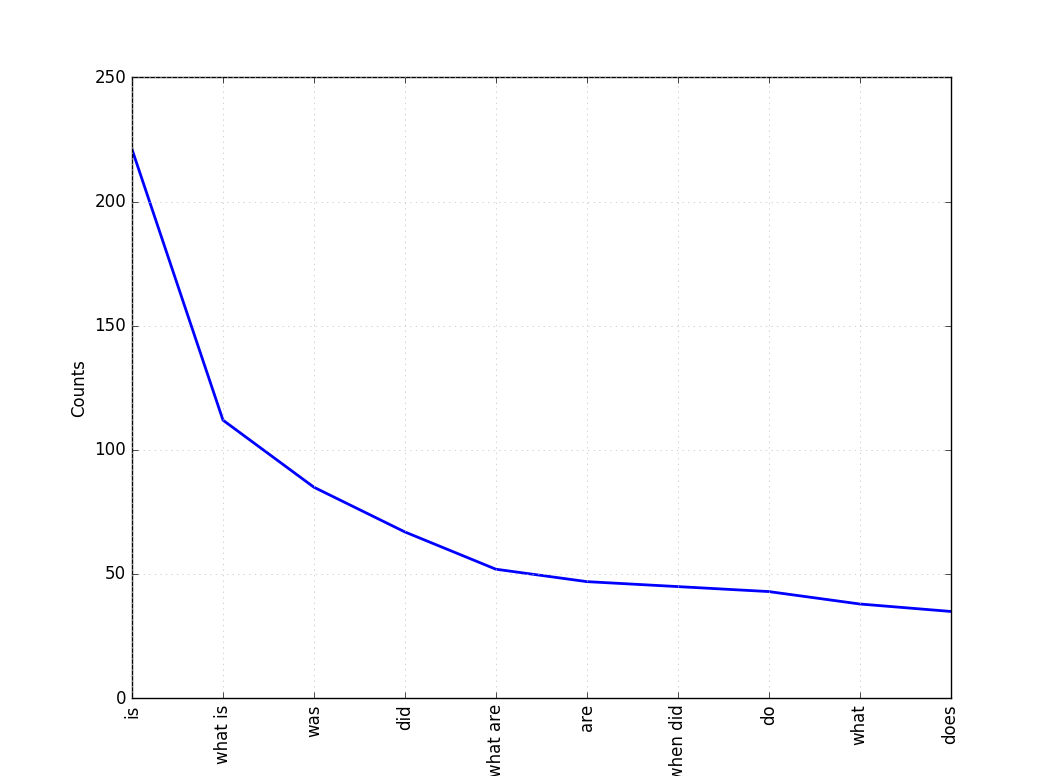
\includegraphics[width=400px]{figures/qtypes.png}
\end{figure}

Table \ref{fig:datastat} shows selected statistics on the corpus.

\section{Methods}

\subsection{Empirical Analysis of \textit{wh}-Forms}

I focus on \textit{what} questions (\textit{what is}, and \textit{what} VERB) to determine if any patterns exist in the spine forms for these questions.

\paragraph {Extracting Question Forms} I use the following regular expression
\begin{equation} \label{eq:qre}
\begin{split}
\text{\textbackslash b(who|what|where|why|when|which|how|many|can|}\\
\text{is|are|do|does|did|were|was|will|has|have|had)\textbackslash b}
\end{split}
\end{equation}

To find all question and tense words (including \textit{many}) in a question.  It's imperfect but it works fairly well at making a rough question class clustering.  After this, I build a frequency distribution over all observed question, tense tuples.  The top 10 of these classes are displayed in Figure \ref{fig:qtypes}.

In addition, I collect examples for the top 10 question classes.  Some selected results of which are dispalyed in the table in Figure \ref{fig:whatqs}.

\paragraph{Analyzing Answer Forms}

Many of these \textit{what} QA problems have the structure of the question ``What is Colomb's Law''.

\begin{multicols}{2}
\begin{dependency}[edge horizontal padding=5pt]\begin{deptext}[column sep=0.1cm]WP \& VBZ \& NNP \& POS \& NN \& .\\What \& is \& Coulomb \& 's \& Law \& ?\\\end{deptext}\depedge{1}{2}{cop}\depedge{5}{3}{nmod:poss}\depedge{3}{4}{case}\depedge{1}{5}{nsubj}\depedge{1}{6}{punct}\deproot{1}{root}\end{dependency}


\begin{dependency}[edge horizontal padding=5pt]\begin{deptext}[column sep=0.1cm]NNP \& POS \& NN \& VBZ \& NNP\\Coulomb \& 's \& Law \& is \& $x^\prime$.\\\end{deptext}\depedge{3}{1}{nmod:poss}\depedge{1}{2}{case}\depedge{5}{3}{nsubj}\depedge{5}{4}{cop}\deproot{5}{root}\end{dependency}

\end{multicols}

In this example, the left form is the original question, and the right form is an expected answer parse.  We can see, in the question on the left, the subject of the sentence is the ``Law'' of which ``Coulomb'' possesses.  Therefore, the logical form for the thing in which we are searching for takes the form

\begin{equation}
\lambda x.\ \text{ROOT}(n_0) \wedge \text{x}(n_i) \wedge nsubj(n_0, n_i)
\end{equation}

In the question Formula above, $x$ represents the concept we are searching for (i.e. \textit{what} is $x$?; in this example: \textit{what is Coulomb's Law?}).  On the right we have the answer whose parse tells us Coulumb's Law is $x^\prime$!  Therefore the form we are looking for must depend on both $x$ and $x^\prime$.

\begin{equation} \label{eq:search_what}
\lambda x.\ \lambda x^\prime.\ \text{ROOT}(n_0) \wedge \text{x}(n_i) \wedge \text{$x^\prime$}(n_j) \wedge root(n_0, n_j) \wedge nsubj(n_j, n_i) 
\end{equation}

Does exactly this.  This query can be used to search for answers (those $x^\prime$ who satisfy \ref{eq:search_what}).

\subsubsection{IR Limitations} Not all questions or answers are created equal.  In natural language one can phrase things in an infinitude of different ways.  In syntactic structure alone, many variations of the above question and answer forms may be used, all refering to the same information. Morphologically, the evaluation is even more bleak; synonyms for words abound, and if no way to deal with these exist, one cannot possibly hope for a system to handle any of them.  So these two issues limit the ability of this mapping, where, although there may exist a singular semantic concepts for both question and answer, there is an infinitude of extensions of these, in practice.  Another problem is coreference, which is not handled in this system.

\subsection{Testing the Plausibility of Formula \ref{eq:search_what}}

By enumerating many possible answer forms, I hypothesize, it may be possible to achieve baseline question answering for this form of \textit{what} question.  I test the plausibility of this hypothesis by executing Formula \ref{eq:search_what} on a subset of my corpus.

\paragraph{Preparing the Data}

I prepare the \textit{Musical instruments} set of the corpus by parsing sentences in all documents related to the musical instruments (see Table \ref{fig:datastat} for full list).  I tokenize the raw text into sentences and run my constituency and dependency parsers on each in sequence.  The result is a set of dependency graphs with which I convert to a more explicit logical form.

\paragraph{Preparing the Test Data}

I prepare the questions by searching for \textit{what} questions among the relevant set of questions in the corpus.  I compile the matched results into a set of 16 questions to test (see Figure \ref{fig:test_data} for full list).

\paragraph{IR Search}

I search for potential solutions to Formula \ref{eq:search_what} using the compiled list of dependency forms generated from the prepared data.  The search algorithm progresses by looking for matches in the terms of the dependency formula given the current $x$ and $x^\prime$.  When a match is found, it is placed into frequency distribution.  It is quite possible that the parse might return many matches.  In practice, the match with the most coverage of $x$ dependents and the highest frequency is most preferred.  However, in this pilot test, I take a more simplistic approach and return only perfect matches.

\begin{figure}
\caption{The test data used for the pilot test of \text{what} QA; the questions are from the \textit{Musical Instruments} set (see: Table \ref{fig:datastat} for full list). \label{fig:test_data}}
\begin{tabular}{|l|p{10cm}|p{2cm}|}
\hline
Topic & Question & Answer \\ \hline
Cymbal & What part of the cymbal is the bell?  & The center of a Cymbal \\ \hline
Drum & What is the second biggest factor affecting the sound produced by a drum?   & tension \\ \hline
Flute & What is the earliest extant transverse flute?  & it dates from 433 BC \\ \hline
Flute & What is the earliest extant transverse flute?  & Chi \\ \hline
Flute & What material is a chi flute fashioned from?  & lacquered bamboo \\ \hline
Flute & What is the most basic form of the flute?  & Open tube which is blown like a bottle \\ \hline
Guitar & What is the bridge used for?  & The transfer of string vibrations. \\ \hline
Guitar & What is located at the end of the guitar neck furthest from the body?  & headstock \\ \hline
Guitar & What is the point called that is bolted or glued to the body of the guitar?  & Neck Joint \\ \hline
Piano & What is the middle pedal called on grand pianos?  & sostenuto pedal \\ \hline
Piano & What is the sustain pedal called?  & damper pedal \\ \hline
Trumpet & What is the earliest date of the trumpet?  & 1500 BC \\ \hline
Trumpet & What is a trumpet constructed of?  & brass tubing \\ \hline
Trumpet & What shape is a trumpet bent into?  & oblong \\ \hline
Violin & What is a violin called informally? & Fiddle \\ \hline
Violin & What is a person that makes or repairs violins called? & Luthier \\ \hline
\end{tabular}
\end{figure}

\begin{figure}
\caption{Examples of \textit{what} questions \label{fig:whatqs}}
\begin{tabular}{|l|l|l|}
\hline
what is the most common color of ants? & what happened in 1894? \\ \hline
what family is the panda a part of? & what religion holds majority in melbourne? \\ \hline
what is coulomb's law? & what led pascal to his religious conversion? \\ \hline
what is panda diplomacy? & what happened in 1810? \\ \hline
what's the population of kuala lumpur? & what happened in 1894? \\ \hline
\end{tabular}
\end{figure}

%------------------------------------------------

\section{Results}

I used Formula \ref{eq:search_what} to find potential answers to queries.  I extract sentences which answer the question, then filter from this result $x^\prime$.

Full results will be available in the next release of this paper, but the initial results are promising; the system was able to extract the correct answer to ``What is the middle pedal called on grand pianos?'' (``sostenuto pedal'').  As stated before, I will complete these tests and more for the next release.

I suspect however, that the system will not be able to answer all of these questions correctly.  The structural variations in the questions alone are enough to upset the model, and deeper analysis into the structure of \textit{what} question and answer forms will definitely help the results quality, as a few of my other runs on the test data were not able to turn up any results at all.

\section{Discussion \& Timeline}

Over the next few weeks, attempts will be made at answering factual $wh$-questions using the corpus and constructed QA pairs.  However, I am not interested in solving QA in this paper;  this is an unreasonable goal.

I am interested in (i) how this formalism can be used in a system that derives logic from natural language itself;

(ii) how spine semantics can be combined with statistics to learn models for QA;

(iii) how probabilistic models can derive candidate logical forms for answers from logical forms of questions in the dependency formalism;

(iv) training a model on QA pairs themselves, applying ML to discover mappings;

and (v) IR over the sentences can derive actual answers.

Unfortunetly, not all of these interests can be satisfied in this paper.  Here is my plan for the coming weeks:

\begin{itemize}

\item \textbf{I will futher develop my method}.  I realize much work needs to go into developing my method.  For each type of question, my goal is to create mappings between natural language question forms to candidate queries (underspecified logical forms $F(x)$ that are satisfied only if $x$ is the answer to the query).

\item \textbf{I will continue to run experiments on the corpus}.  I know my system will be incapable of answering questions requiring inference, or resolving instances of coreference; these are subjects for another study.  However, for the system I do have, I will test it by attempting to answer $wh$-questions in the corpus; Finally, I will report my results.

\end{itemize}

%----------------------------------------------------------------------------------------
%	REFERENCE LIST
%----------------------------------------------------------------------------------------

%\begin{multicols}{2}
\begin{thebibliography}{9} % Bibliography - this is intentionally simple in this template

\bibitem{guo08}
Yuqing Guo, Josef van Genabith, Haifeng Wang (2008)
\newblock Dependency-Based N-Gram Models for
General Purpose Sentence Realisation
 
\end{thebibliography}
%\end{multicols}

%----------------------------------------------------------------------------------------

\end{document}
